\documentclass{article}
\usepackage[margin=0.8in]{geometry}

\usepackage{hyperref}
\usepackage{minted}
\usepackage{pdfpages}
\usepackage{graphicx}
\usepackage{listings}

\lstset{
	numbersep=8pt, 
	frame = single, 
	framexleftmargin=15pt}

\begin{document}
\hypersetup{pageanchor=false}
\begin{titlepage} % Suppresses headers and footers on the title page
  \centering % Centre everything on the title page
  
  %------------------------------------------------
  %	Title
  %------------------------------------------------
  \vspace*{0.1\textheight}
  \large{EEL 5721 -- Reconfigurable Computing}\\
  \vspace{0.0025\textheight}
  
  \huge{Lab 0 -- VHDL Tutorial}
  \vspace{0.025\textheight} % Whitespace between the title and short horizontal rule
  
  \rule{0.3\textwidth}{0.4pt} % Short horizontal rule under the title
  \vspace{0.1\textheight} % Whitespace between the thin horizontal rule and the author name
  
  %------------------------------------------------
  %	Author
  %------------------------------------------------
  \small{By}\\
  \Large \textsc{Nathan Jessurun}\\% Author name
  \vspace{0.04\textheight}
  
  \vspace{0.10\textheight}
  \normalsize{
    \today
  }
  \vfill % Whitespace between the author name and publisher
  
  \rule{\textwidth}{0.4pt} % Thin horizontal rule
\end{titlepage}
\hypersetup{pageanchor=true}
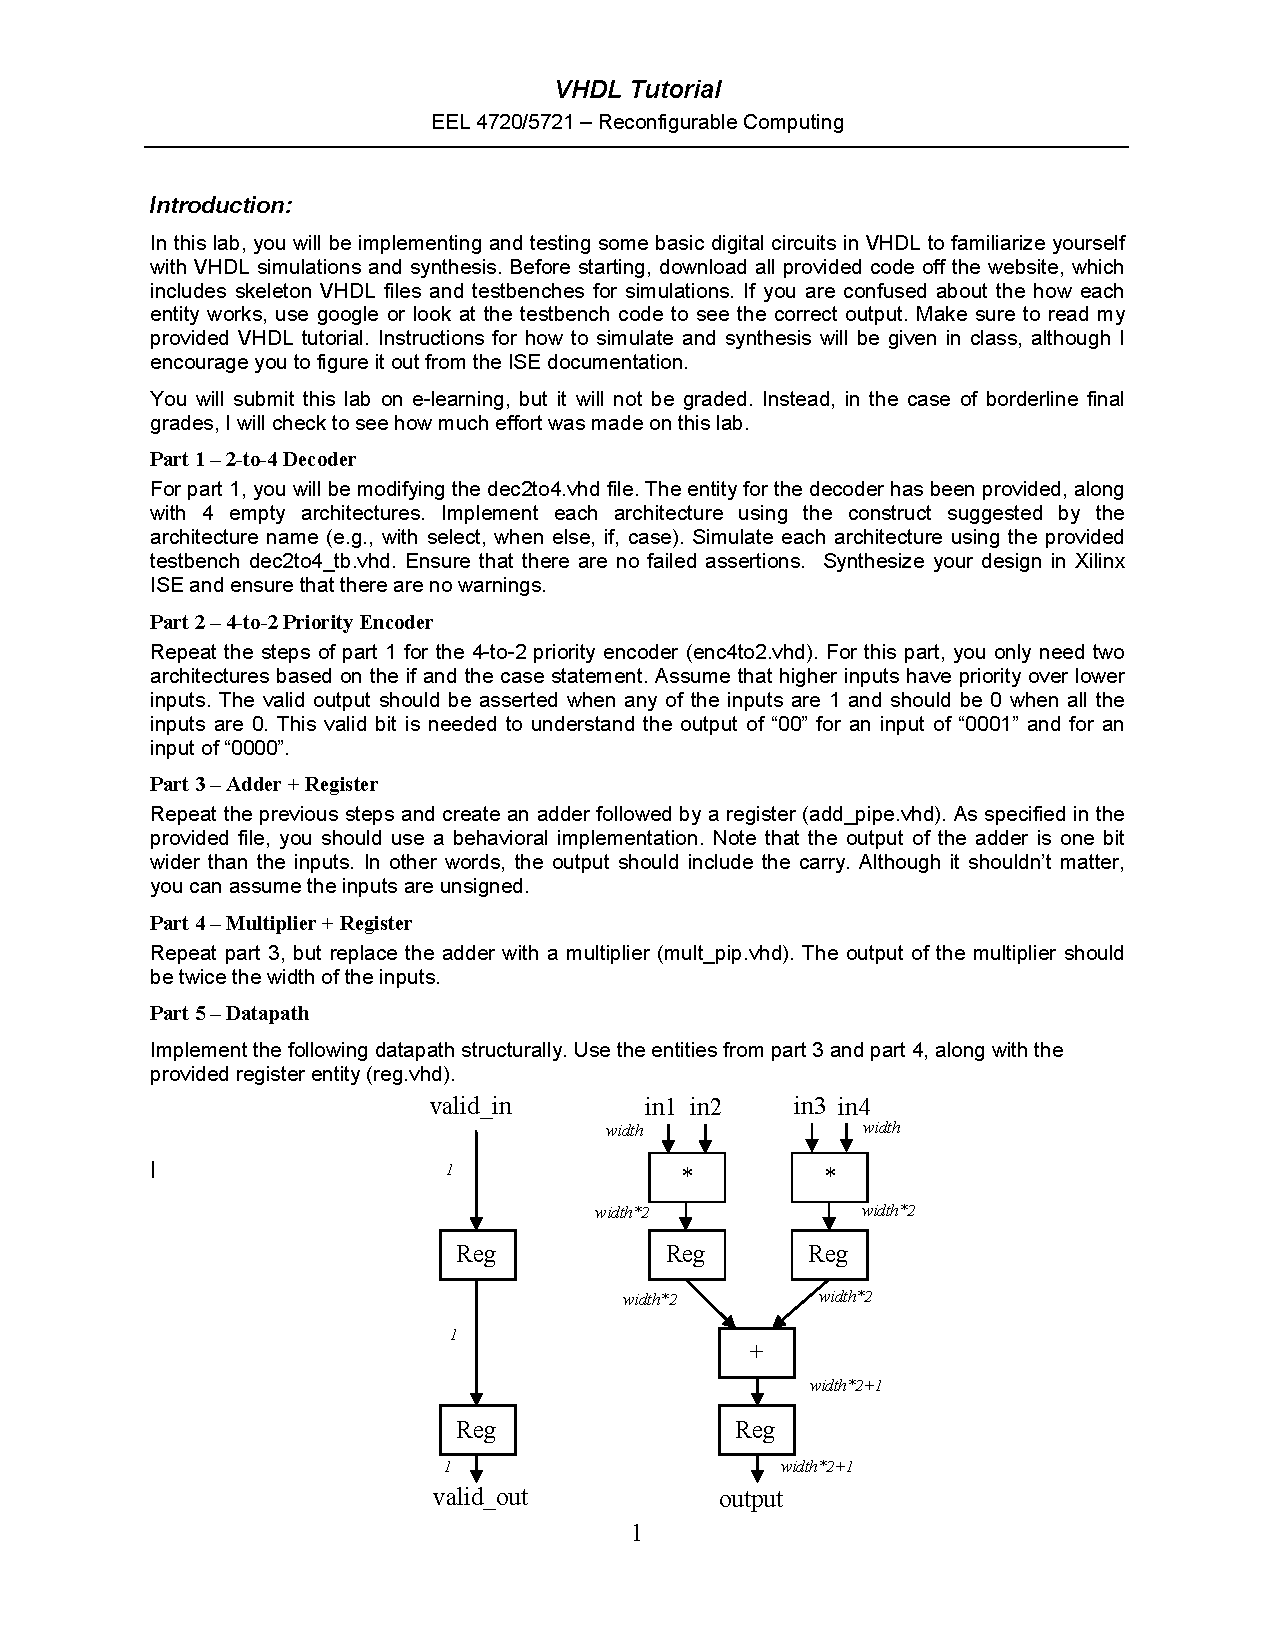
\includepdf{./lab}

\section{Working Simulations}

\subsection{2-to-4 Decoder}
\begin{figure}[H]
	\centering
	\includegraphics[width=\linewidth]{figures/modelsim_2to4Decoder}
	\caption{All architectures properly decode the input signal}
	\label{fig:modelsim2to4decoder}
\end{figure}
\begin{figure}[H]
	\centering
	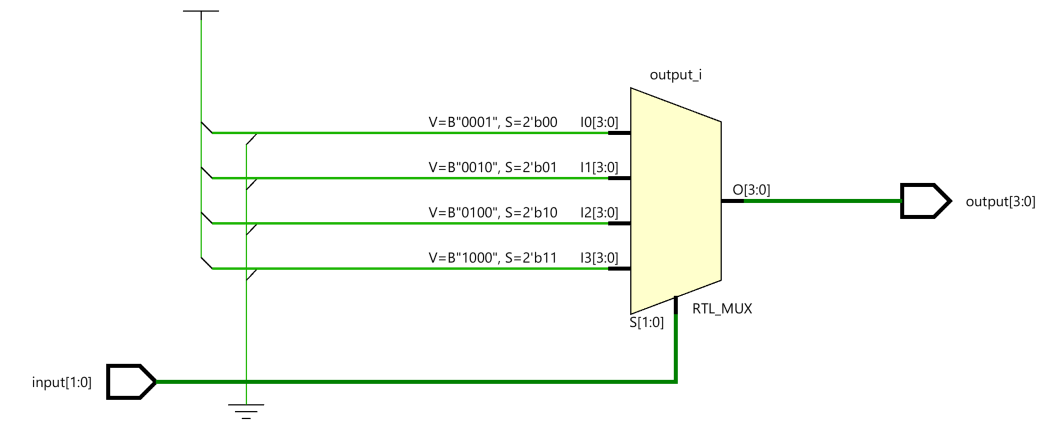
\includegraphics[width=0.5\linewidth]{figures/decoderSchematic}
	\caption{Synthesized schematic correctly indicates a mux implementation}
	\label{fig:modelsim2to4decoder}
\end{figure}

\subsection{4-to-2 Priority Encoder}
\begin{figure}[H]
	\centering
	\includegraphics[width=\linewidth]{figures/modelsim_4To2PriorityEncoder}
	\caption{All architectures properly encode the input signal}
	\label{fig:modelsim4to2priorityencoder}
\end{figure}

\subsection{Add Pipeline}
\begin{figure}[H]
	\centering
	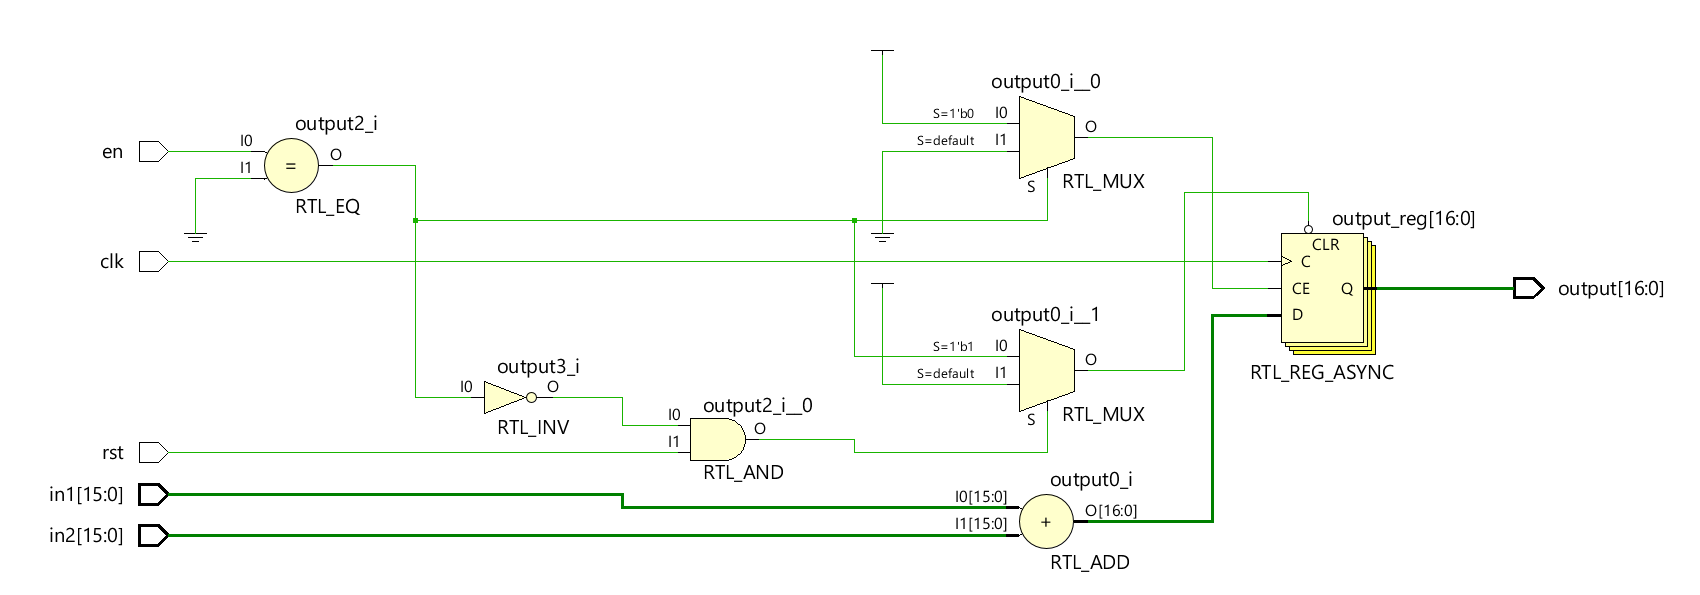
\includegraphics[width=\linewidth]{figures/add_pipe}
	\caption{Add pipeline has no inferred latches}
\end{figure}

See the tabulated simulation results below indicating proper behavior when the `done' bit indicate the final computation has appropriately propagated:
\lstinputlisting[firstline=0,lastline=33]{../modelsim/add_pipe_tb.lst}

\subsection{Mult Pipeline}
\begin{figure}[H]
	\centering
	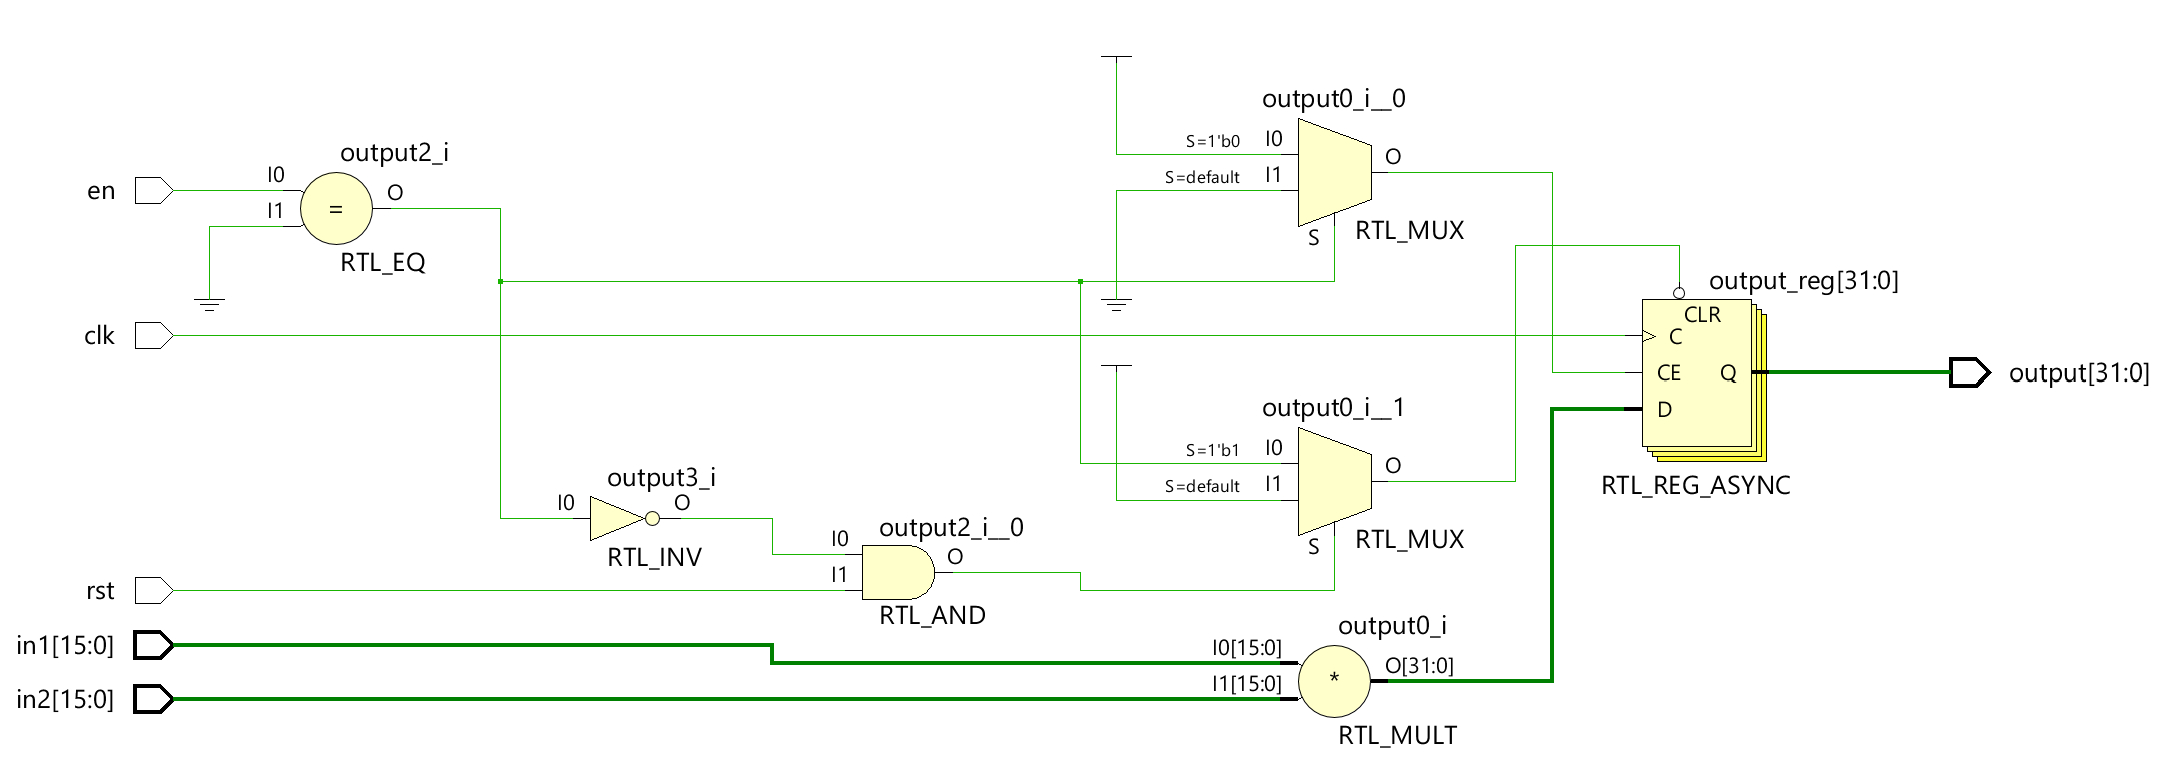
\includegraphics[width=\linewidth]{figures/mult_pipe}
	\caption{Mult pipeline has no inferred latches}
\end{figure}

See the tabulated simulation results below indicating proper behavior:
\lstinputlisting[firstline=0,lastline=33]{../modelsim/mult_pipe_tb.lst}


\subsection{Datapath Pipeline}
\begin{figure}[H]
	\centering
	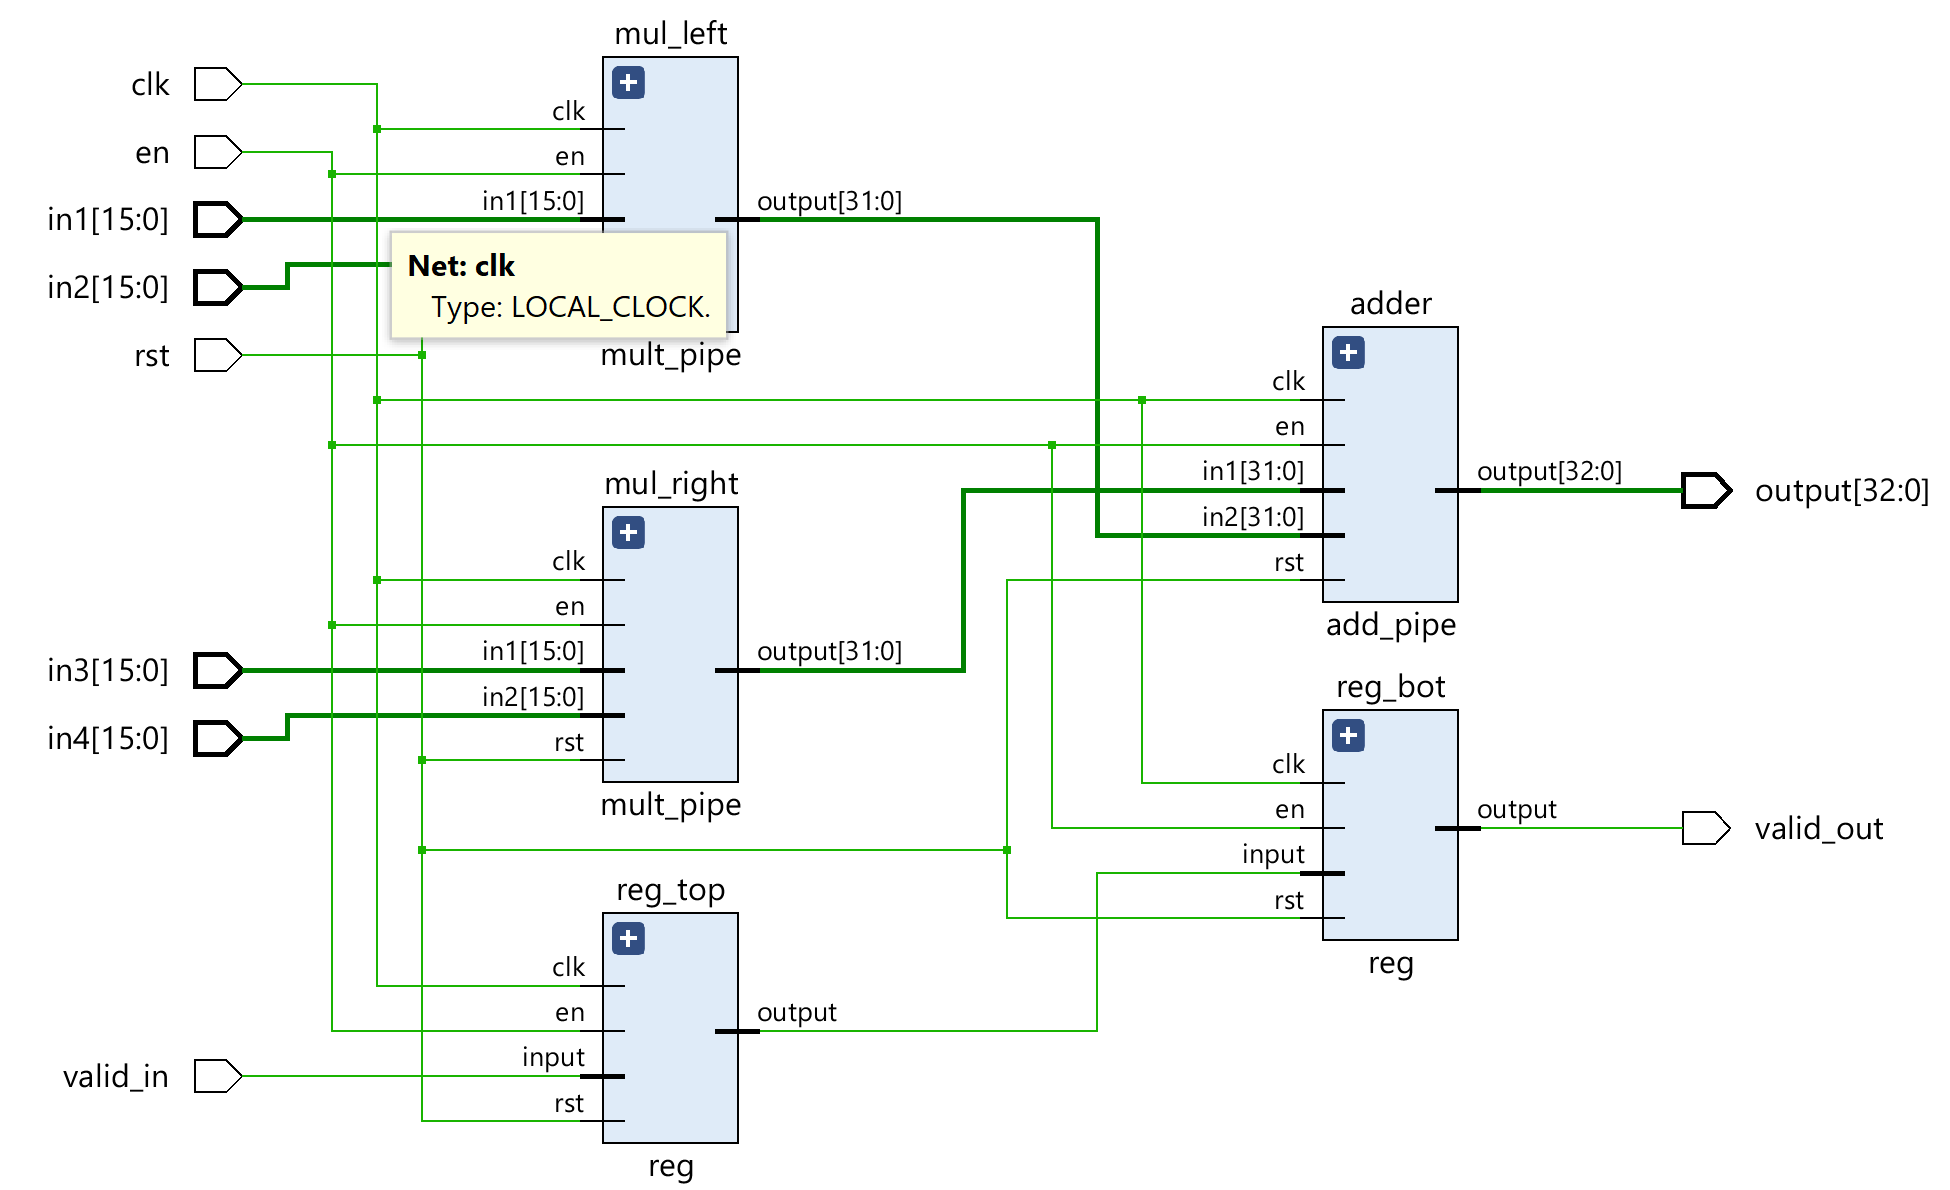
\includegraphics[width=\linewidth]{figures/datapath}
	\caption{Datapath is correctly synthesized as an architectural diagram}
\end{figure}

See the tabulated simulation results below indicating proper behavior:
\lstinputlisting[firstline=0,lastline=33]{../modelsim/datapath_tb.lst}



\section{Code Listings}
Per instructions, all code files (and test bench listings) are zipped along with the project report.
\end{document}